\section{Data Description}
Standartox constitutes a collection of 600,000 quality checked ecotoxicological test results comprising roughly 8000 distinct chemicals and 8000 taxa that allows for the retrieval of single toxicity equivalents. It is build on the ECOTOX database \citep{usepa_ecotox_2019} and the data is processed in order to clean and harmonise entries to retrieve comparable toxicity endpoints. Subsequently, filter and aggregation methods are provided to allow for the retrieval of single toxicity equivalents for specific test parameter combinations. The underlying ECOTOX database is released quarterly and provides on average \input{article/values/publish_rate.txt} (2014 - 2019) new test results with each release. Standartox is build directly after each new ECOTOX release in an automated way and therefore incorporates new data steadily. To guarantee reproducibility, users can choose which Standartox version to access. Users can reach Standartox via an web app and an R-package (standartox) that accesses an application programming interface (API) providing the possibility of scriptable requests.

\subsection{Filters}
The data can be restricted to three endpoint groups XX50, LOEX and NOEX, conflating commonly used endpoints such as half maximal effective concentrations (EC\textsubscript{50}), no observed effect levels/concentrations (NOEC/L), as well as lowest observed effect levels/concentrations (LOEC/L) respectively (Table \ref{tab:endpoints-conflate}) (Fig. \ref{fig:stx-parameters}A). Standartox allows the ecotoxicity data to be filtered to 23 distinct effect groups (e.g. mortality, population, growth) (Fig. \ref{fig:stx-parameters}B) and concentration types (e.g. formulation, active ingredient). In addition to these test-specific parameters Standartox data entries can be filtered according to chemical-specific parameters such as, the CAS number and five chemical classes (e.g. pesticides, metals, drugs), commonly used in ecotoxicology (Fig. \ref{fig:stx-parameters}C). Furthermore, the Standartox data can be refined to organism-specific parameters, such as the organism habitat (e.g. freshwater, marine, terrestrial) (Fig. \ref{fig:stx-parameters}E), the occurrence regions (e.g. Europe, South America) (Fig. \ref{fig:stx-parameters}F) of the organisms as well as different taxonomic levels. Additionally users can refine the results to specific test durations (in hours).

\begin{figure}[h!]
    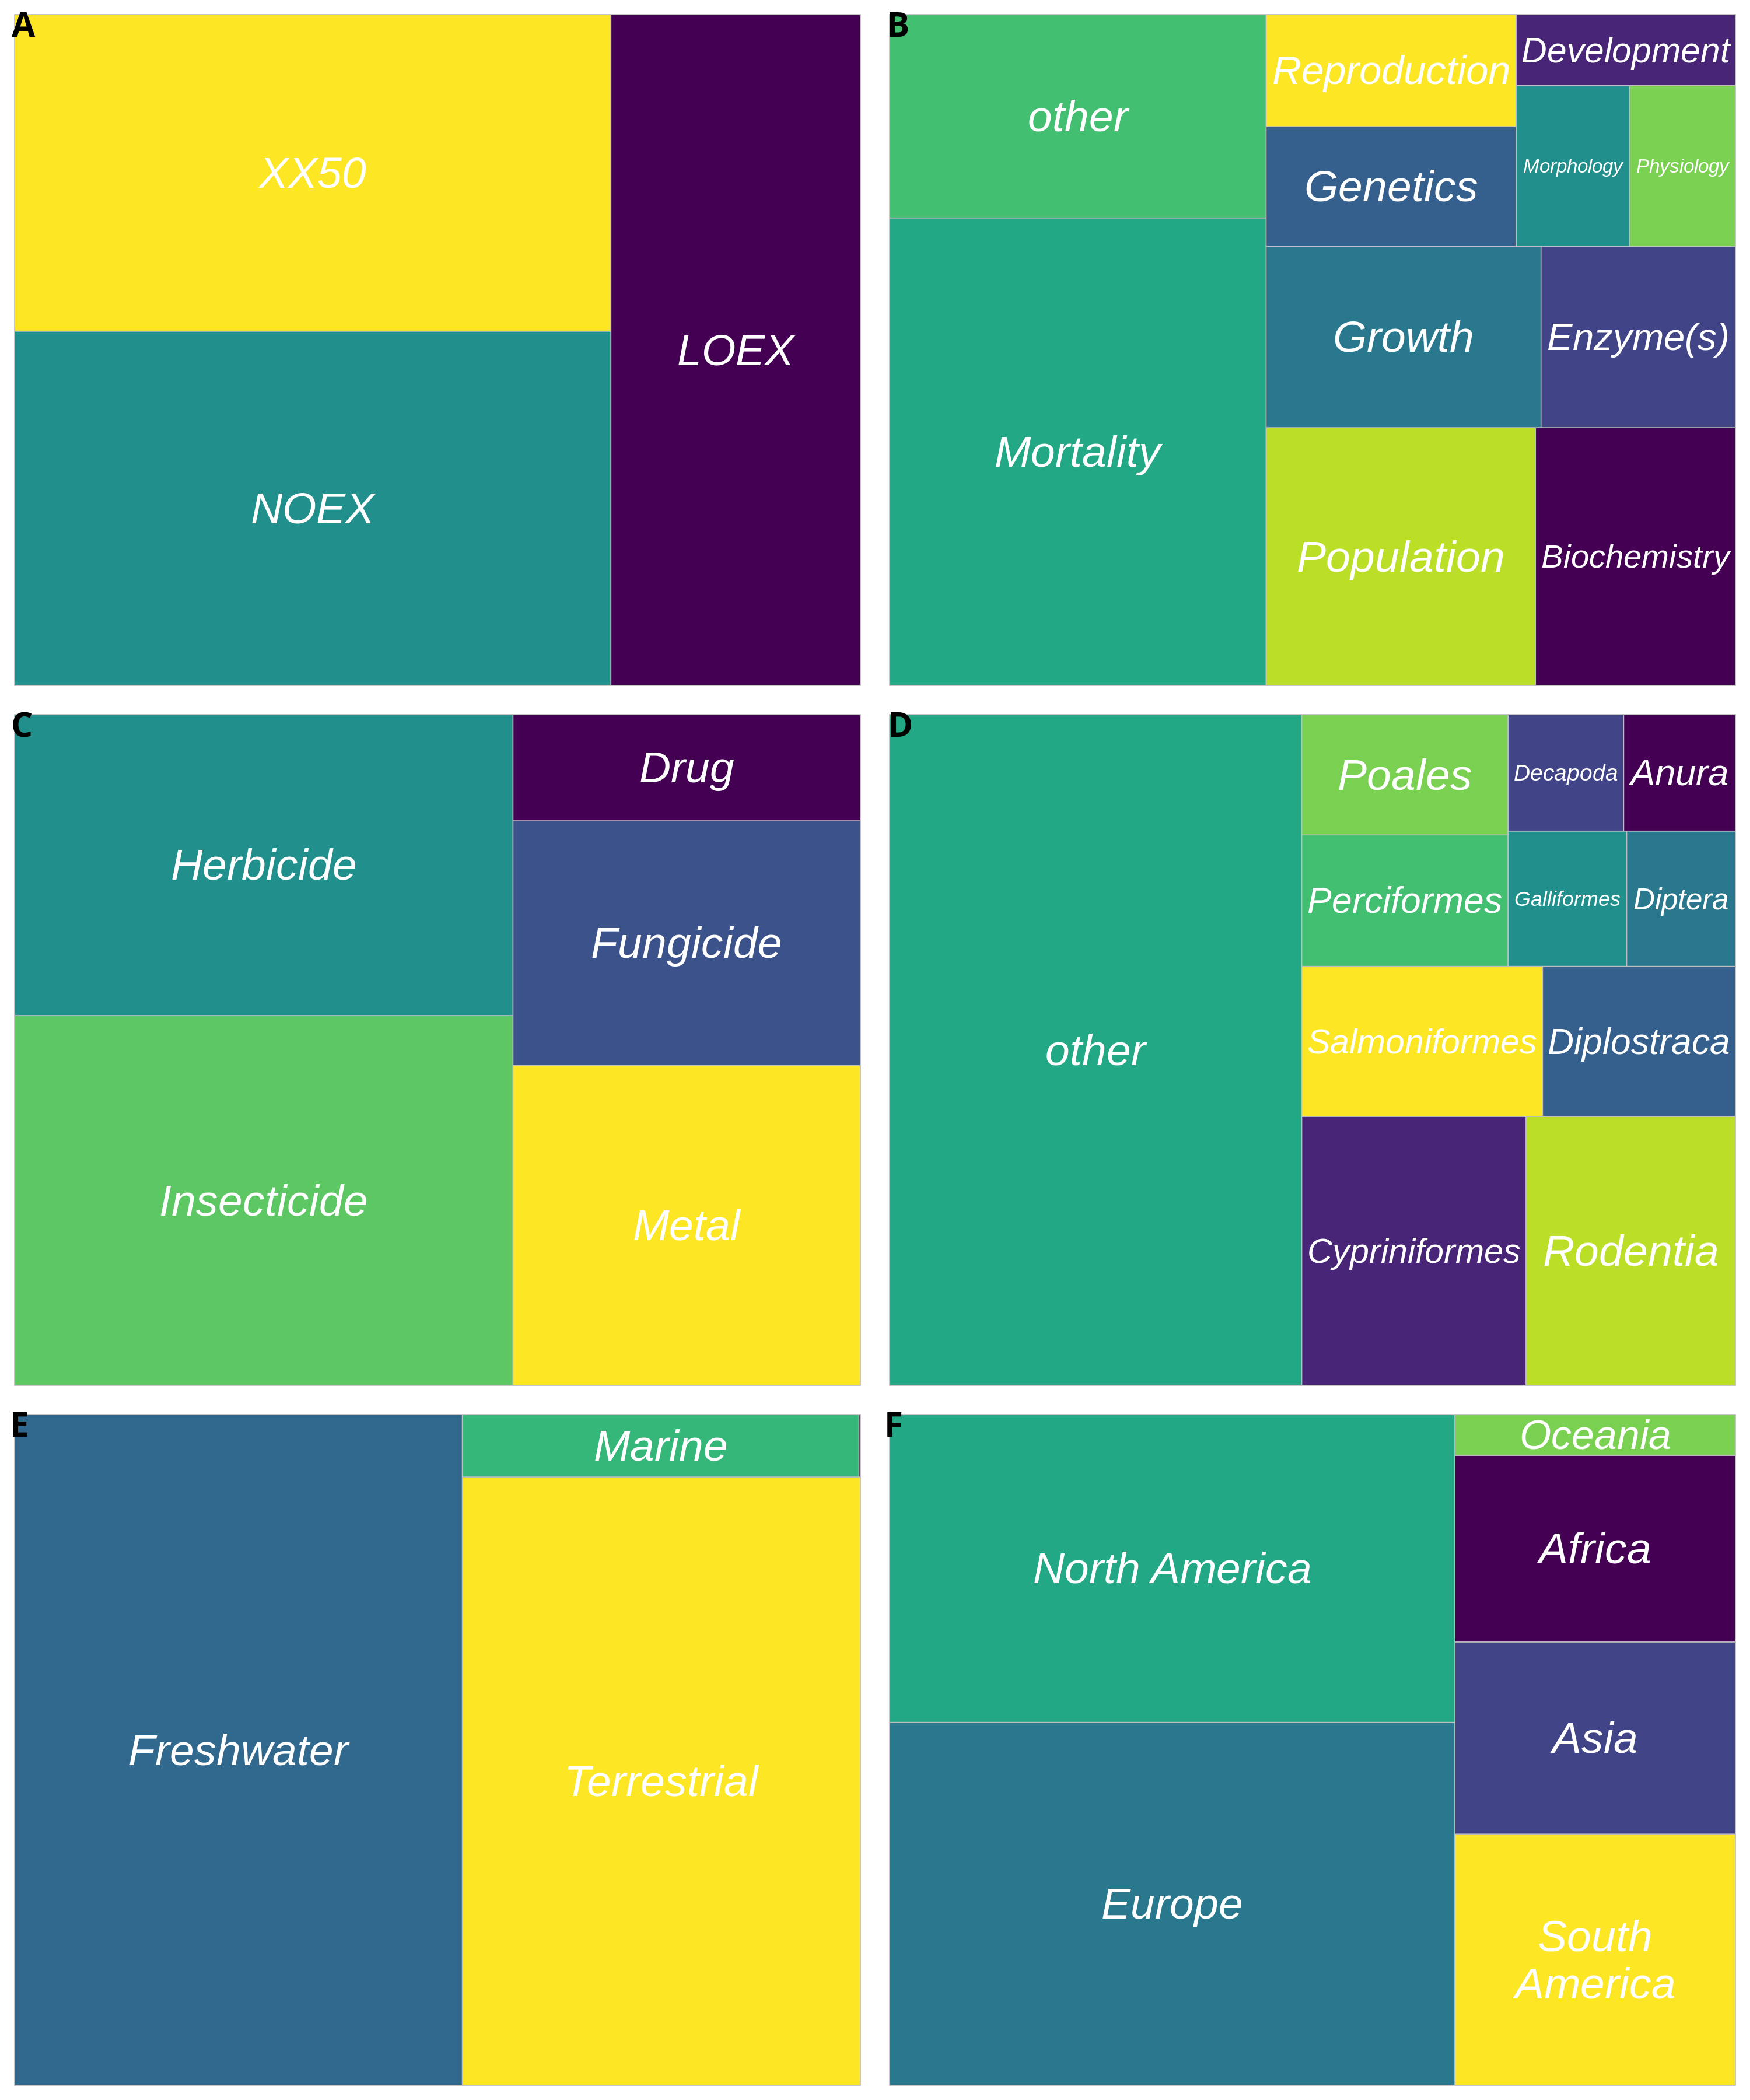
\includegraphics[width=1.0\textwidth]{article/figures/standartox_parameters.png}
    \caption{Share of 10 most occurring entries for the parameters endpoint (A), effect (B), chemical class (C), taxonomic order (D), organism habitat (E) and organism occurrence region (F) in Standartox.}
    \label{fig:stx-parameters}
\end{figure}

\subsection{Aggregation}
In order to reduce multiple ecotoxicity values for individual chemical-species combinations and to solve the associated problem of which value to choose for CRA, Standartox introduces aggregation methods that enable the derivation of single ecotoxicity values. This aggregation step is important because multiple test results exhibit highly variability in chemical risk assessment (CRA) due to several factors, such as differences in the susceptibility of different taxa to a chemical (Fig. \ref{fig:stx-variability}A), test results variability of one and the same taxon and chemical due to different test durations (Fig. \ref{fig:stx-variability}B) as well as variability caused by unexplainable factors, due to different laboratories, physiological differences between organism populations or other unaccounted variation (Fig. \ref{fig:stx-variability}C). Standartox calculates the minimum, the maximum and the geometric mean as aggregates from the filtered data set for each chemical. The geometric mean is preferred in comparison to the arithmetic mean, since it is considerably less influenced by outliers and is suitable for skewed data. Also, the geometric mean is preferable over the median, since the median completely ignores the influence of large or small values, making it unreliable for small data sets. In the course of the aggregation process, outliers that exceed 1.5 times the interquartile range are flagged to caution Standartox users. However, since the geometric mean is not strongly influenced by such entries, they are not removed.

\begin{figure}[h!]
    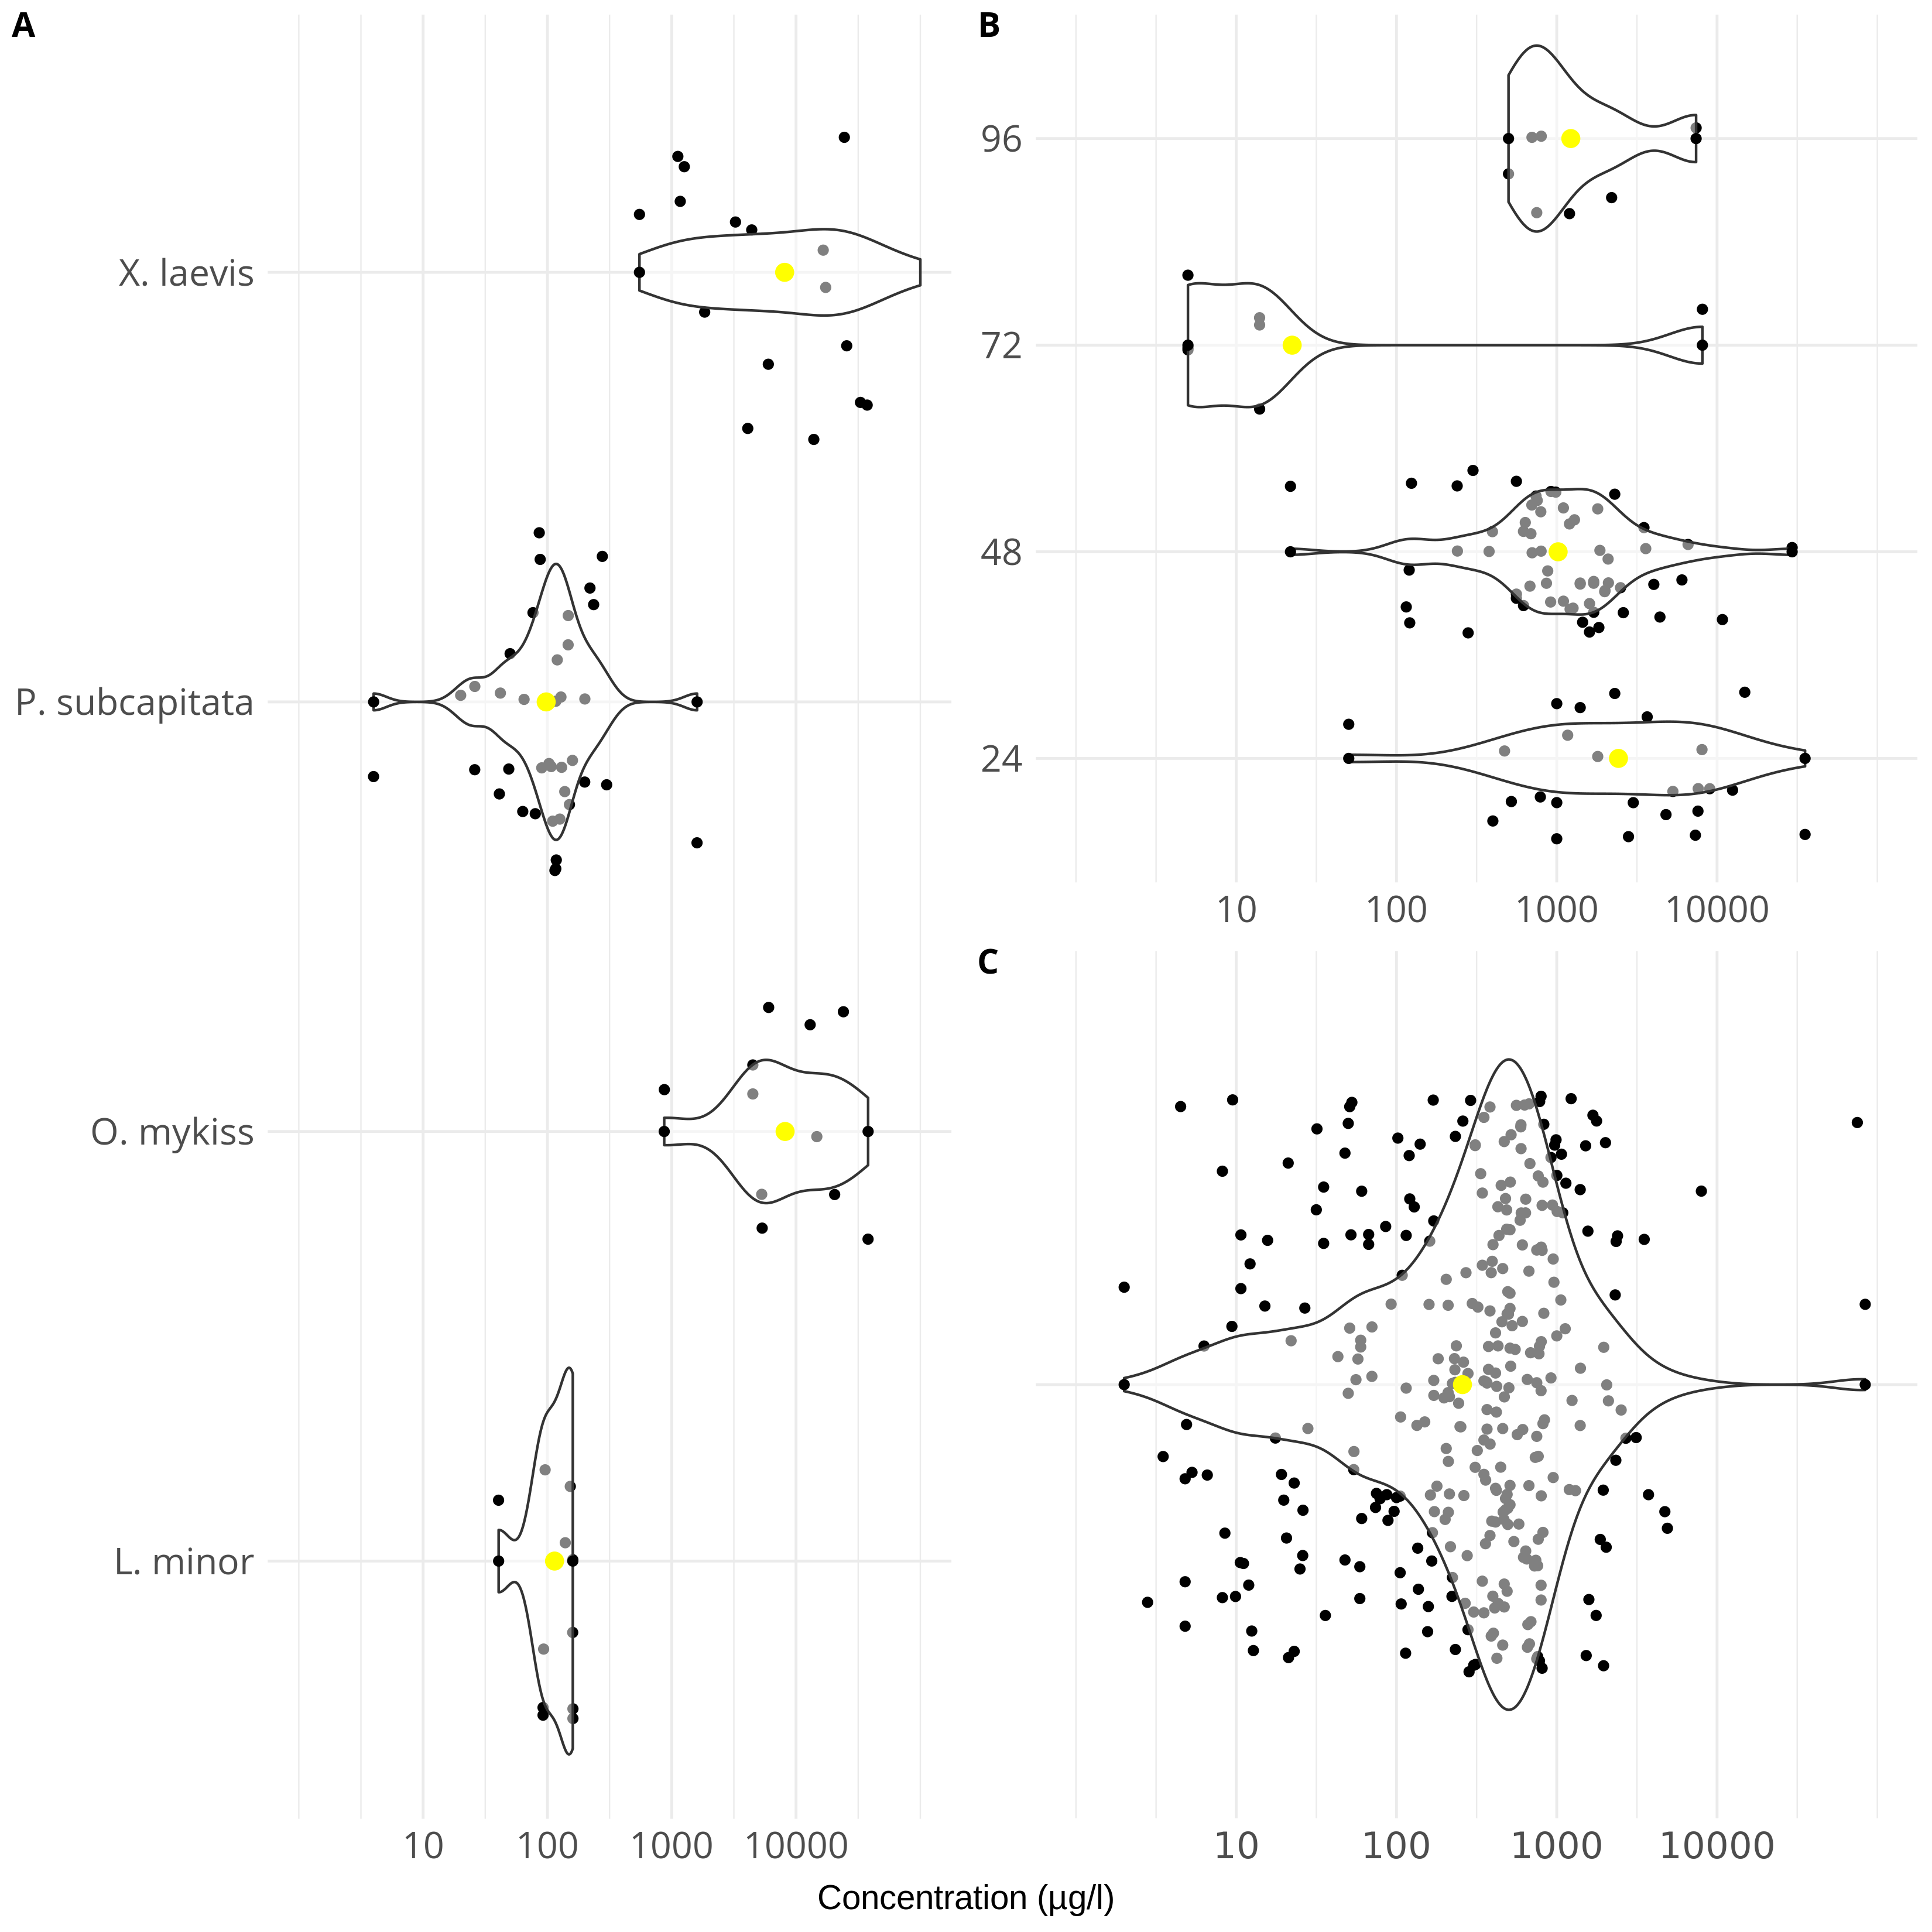
\includegraphics[width=1.0\textwidth]{article/figures/results_variability.png}
    \caption{Variability of test results (EC\textsubscript{50}) in Standartox due to (A) the susceptibility of different taxa (i.e. \textit{Xenopus laevis}, \textit{Pseudokirchneriella subcapitata}, \textit{Oncorhynchus mykiss}, \textit{Lemna minor}) to the chemical atrazine tested for 96h, due to (B) different durations of tests of zinc sulfate on \textit{Daphnia magna} and due to (C) un-accountable variability of cupric sulfate tested on \textit{Pimephales promelas} for 96h. Yellow dots depict Standartox approximations and black and gray dots show un-aggregated values for each group.}
    \label{fig:stx-variability}
\end{figure}

\subsection{Accuracy Assessment}
In order to validate Standartox results we compared the outputs to values from other databases. Since 2006, the PPDB provides validated ecotoxicological information on pesticides \citep{lewis_international_2016}. 91 \% of the Standartox geometric mean aggregations lie within one order of magnitude to the manually quality checked PPDB (n=3601) values. Considering only Standartox geometric means for which at least five tests were aggregated, the value increases to 92.7 \%. Similarly, we compared Standartox to ecotoxicity values for \textit{D. magna} from the ChemProp \citep{ufzdepartmentofecologicalchemistry_chemprop_2019} software, which estimates LC\textsubscript{50} values via quantitative structure-activity relationship (QSAR) models \citep{schuurmann_quantitative_2011} and found that (n=179) 95 \% lie within a factor of below one order of magnitude in comparison to the Standartox aggregations. However, the difference is not necessarily an indication of lower quality of these data in Standartox but may also be attributed to the inclusion of consideration of a wider range of test data and conditions as well as variance in the QSAR models, respectively (Figure \ref{fig:standartox_ppdb_diff}).

\begin{figure}[h!]
    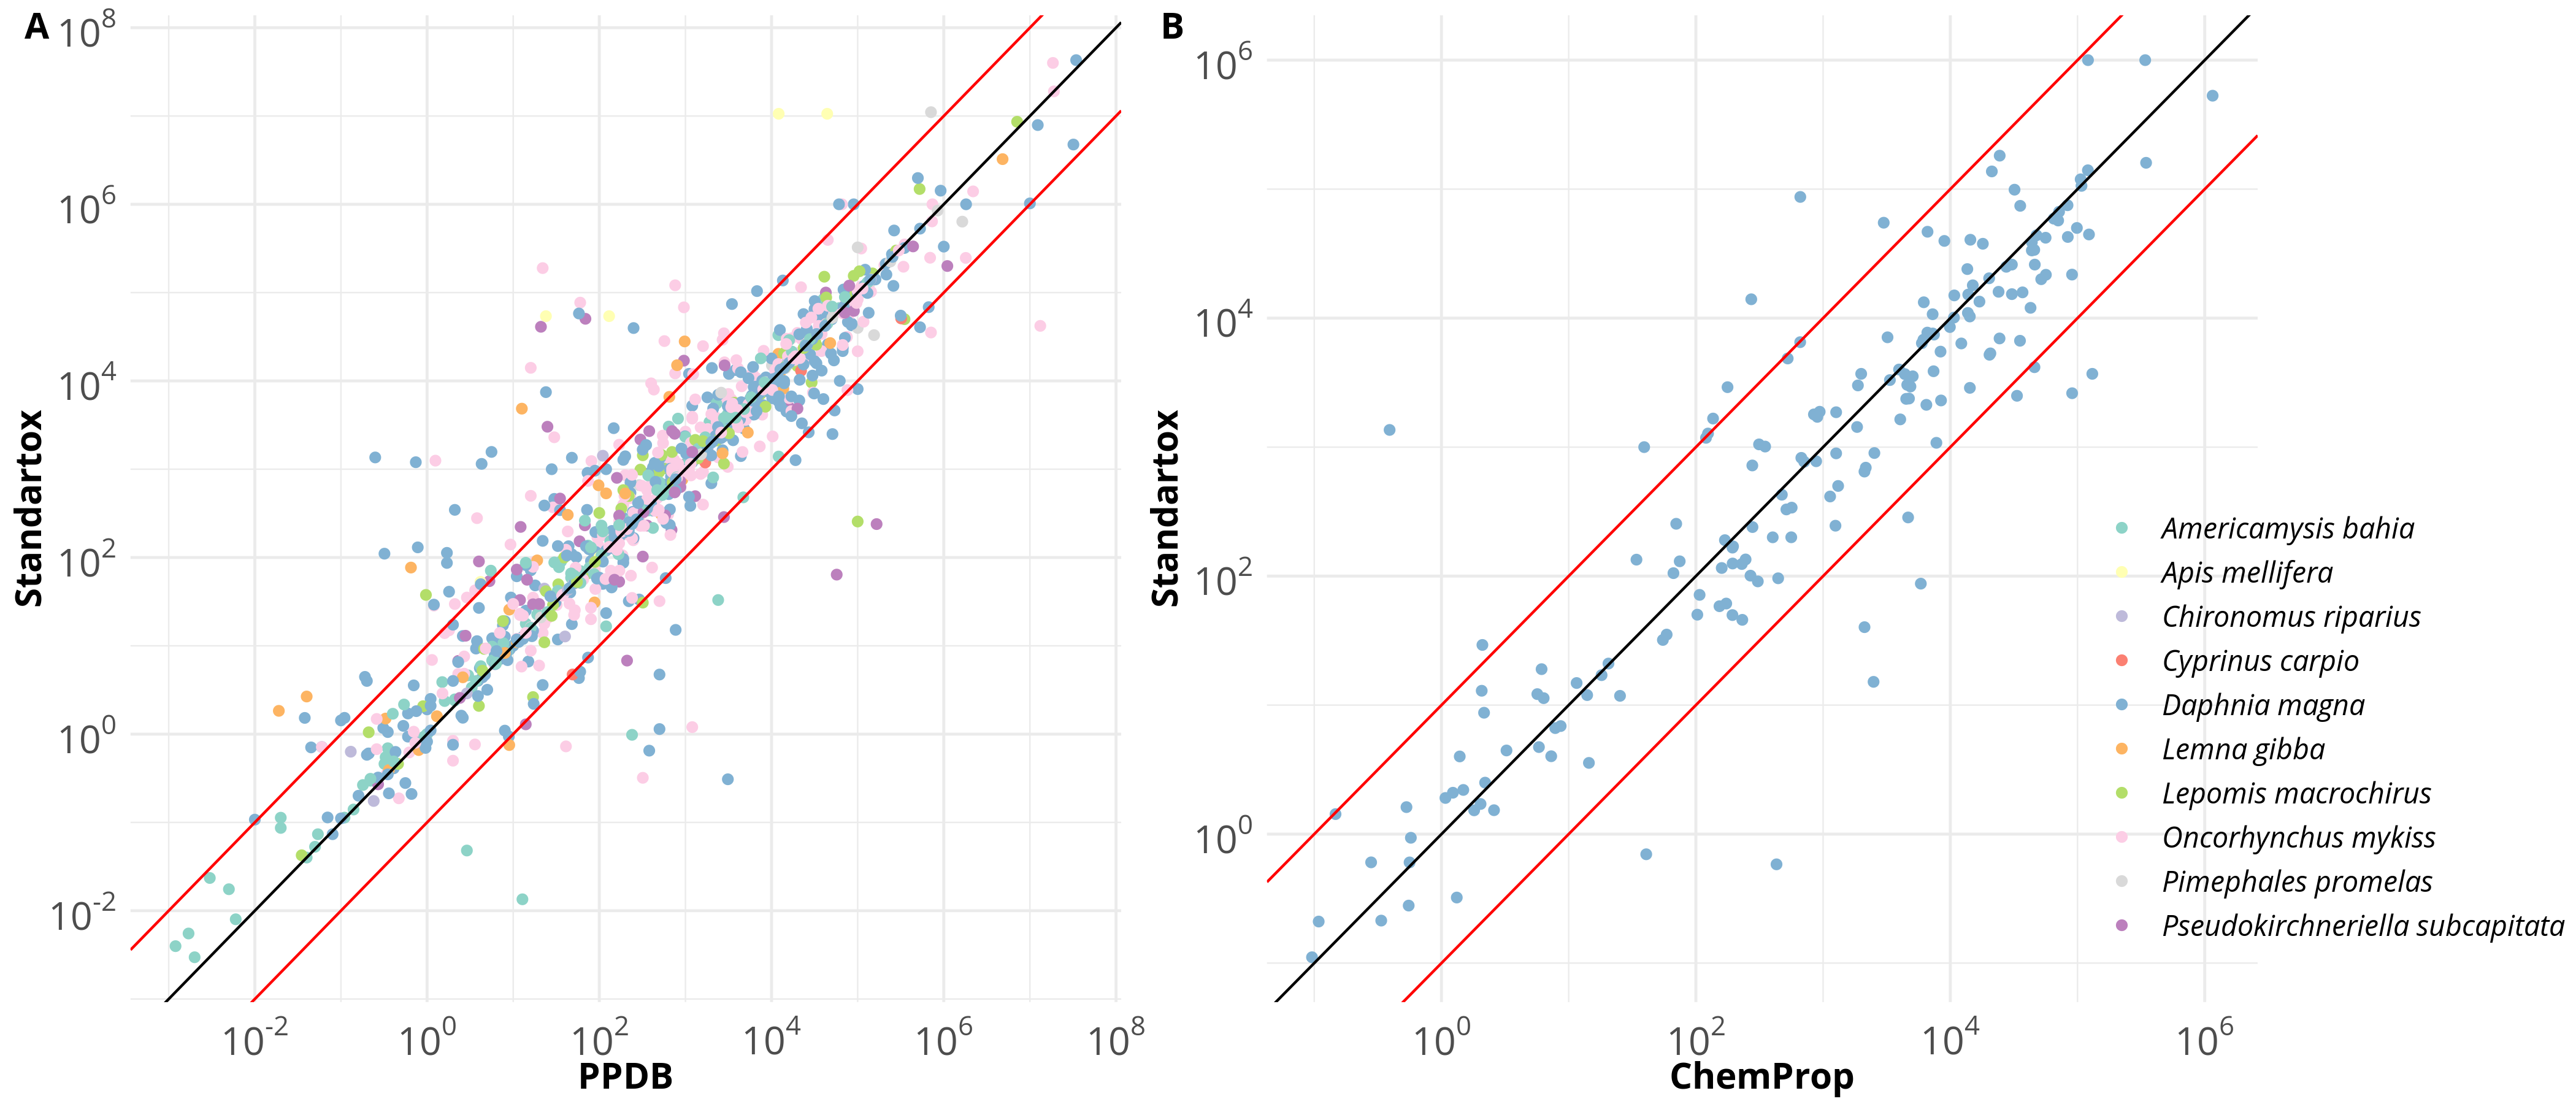
\includegraphics[width=1\linewidth]{article/figures/gg_ppdb_stan_compare_continous.png}
    \caption{Comparison between Standartox and PPDB (A) and read across (B) values. The black lines mark exact coherence and red lines mark a divergence of a factor of 10. Compared organism groups are color coded.}
    \label{fig:standartox_ppdb_diff}
\end{figure}

\subsection{Perspectives}
Other initiatives harmonizing the large number of ecotoxicological test results were also developed recently. They partly aim for overlapping goals, yet have limitations or objectives that differentiate them from Standartox. The Network of reference laboratories, research centres and related organisations for monitoring of emerging environmental substances (NORMAN) focuses on assembling river basin specific pollutants from studies and databases \citep{von_der_ohe_new_2011}. The EnviroTox database \href{https://envirotoxdatabase.org/} which also uses, amongst others the ECOTOX database as an input was recently published \citep{healthandenvironmentalsciencesinstitutehesi_envirotox_2019, connors_creation_2019}. In comparison to Standartox, EnviroTox focuses only on aquatic organisms and uses a qualitative algorithm to derive single ecotoxicity values. For example, they restrict the ecotoxicity data to fish, amphibian, invertebrate and algae taxa only and test durations to be at least above 24 hours. In contrast, Standartox doesn't refine to specific test durations, but leaves it up to the user to decide on such parameters. Besides, they add additional information on toxicity endpoints, such as acute or chronic classifications and mode of action assignments. An action that can also be allocated to the user, since there are several different ways to classify such parameters, especially those mentioned, guaranteeing user flexibility. The EnvirTox database also allows for an aggregation of test results to derive single toxicity values for individual taxa whereas Standartox performs this aggregation for individual chemicals taxa combinations. Comptox, is a web tool published by the EPA which, similar to Standartox allows for filtering test results, the retrieval of additional chemical information and predicting toxicity properties, such as 48 h \textit{Daphnia magna} LC\textsubscript{50} values. However, toxicity predictions are limited to some standard organisms (e.g. \textit{Daphnia magna}), and the tool lacks the possibility to retrieve predicted values in an automated way \citep{williams_comptox_2017}. \citet{petschick_modeling_2019} modeled risk threshold level equivalents for aquatic organisms by using ecotoxicological effect data from the ECOTOX database to support regulation. Along with newly created ecotoxicological databases, methods of how to efficiently store ecotoxicological data are also proposed as can be seen in the MAGIC Knowledge Base \citep{bub_graphing_2019}. Likewise, ideas to create new predictive frameworks in ecotoxicology, incorporating chemical mode of actions and species traits \citep{vandenberg_modeling_2019} together with the recent increase in efforts to compile ecotoxicological test databases clearly emphasizes the need for holistic and automated analyses of large-scale ecotoxicological data. In summary, none of the above mentioned approaches aim for a holistic standardized aggregation method of exposure endpoints for individual chemicals and also lack the possibility for automated and scriptable user requests from common high level programming languages, such as R or Python \citep{pythoncoreteam_python_2020} (Table \ref{tab:database-differences}). Another important feature to improve toxicity estimates is to include a large number of test parameters, such as pH, temperature or conductivity amongst others, since toxicity test results are highly influenced by those \citep{rosenkrantz_influence_2013, li_temperature_2011}. Such information is not included in the aggregation performed by Standartox, since the ECOTOX database only provides sparse records on test parameters. Most frequently provided test parameters (and their percentage) are medium temperature (77\%), pH:56\%, hardness:27\%, dissolved oxygen:18\%, Alkalinity:15\% and salinity:9\%. Others are provided for less than 5\% of the tests. A text-mining approach, iterating through the individual publications could potentially increase this number.

\begin{sidewaystable}
% \begin{table}
    %% table that compares different ecotoxicological databases

%%%% CONTINUE HERE

\begin{sidewaystable}
% \begin{table}
\caption{Different databases that provide ecotoxicological data. Abbreviations: \textbf{ALL:} Most important test parameters, including chemical, taxon, duration for filtering ecotoxicological data are incorporated. \textbf{WEB:} Accessible via a web application through a graphical user interface. \textbf{API:} Accessible via an application programming interface.}
\label{tab:database-differences}
\begin{tabular}{|m{3cm}|m{3cm}|m{2cm}|m{2cm}|m{1cm}|l|}
\hline
Database & Publisher & Filter & Aggregation, Selection & Access & website \\
\hline
Comptox & Environmental Protection Agency & Chemical & no & WEB, file & https://comptox.epa.gov/dashboard \\
\hline
Ecotox & Environmental Protection Agency & ALL & no & WEB, file & https://webetox.uba.de/webETOX/index.do \\
\hline
EnviroTox & Health and Environmental Sciences Institute & ALL & chemical, organism & WEB & https://envirotoxdatabase.org \\
\hline
Etox & Umweltbundesamt & ALL & no & WEB & https://webetox.uba.de/webETOX/index.do \\
\hline
Pesticide Property Data Base (PPDB) & University of Hertfordshire & fixed values & manual selection & WEB, file & https://sitem.herts.ac.uk/aeru/ppdb/index.htm \\
\hline
\textbf{Standartox} & \textbf{this article} & \textbf{ALL} & \textbf{chemical, organism} & \textbf{API, WEB} & \textbf{http://standartox.uni-landau.de} \\
\hline
\end{tabular}
% \end{table}
\end{sidewaystable}



    \caption{Differences of databases that provide ecotoxicological data.}
    \label{tab:database-differences}
% \end{table}
\end{sidewaystable}






